% Options for packages loaded elsewhere
\PassOptionsToPackage{unicode}{hyperref}
\PassOptionsToPackage{hyphens}{url}
%
\documentclass[
]{book}
\usepackage{amsmath,amssymb}
\usepackage{lmodern}
\usepackage{iftex}
\ifPDFTeX
  \usepackage[T1]{fontenc}
  \usepackage[utf8]{inputenc}
  \usepackage{textcomp} % provide euro and other symbols
\else % if luatex or xetex
  \usepackage{unicode-math}
  \defaultfontfeatures{Scale=MatchLowercase}
  \defaultfontfeatures[\rmfamily]{Ligatures=TeX,Scale=1}
\fi
% Use upquote if available, for straight quotes in verbatim environments
\IfFileExists{upquote.sty}{\usepackage{upquote}}{}
\IfFileExists{microtype.sty}{% use microtype if available
  \usepackage[]{microtype}
  \UseMicrotypeSet[protrusion]{basicmath} % disable protrusion for tt fonts
}{}
\makeatletter
\@ifundefined{KOMAClassName}{% if non-KOMA class
  \IfFileExists{parskip.sty}{%
    \usepackage{parskip}
  }{% else
    \setlength{\parindent}{0pt}
    \setlength{\parskip}{6pt plus 2pt minus 1pt}}
}{% if KOMA class
  \KOMAoptions{parskip=half}}
\makeatother
\usepackage{xcolor}
\usepackage{color}
\usepackage{fancyvrb}
\newcommand{\VerbBar}{|}
\newcommand{\VERB}{\Verb[commandchars=\\\{\}]}
\DefineVerbatimEnvironment{Highlighting}{Verbatim}{commandchars=\\\{\}}
% Add ',fontsize=\small' for more characters per line
\usepackage{framed}
\definecolor{shadecolor}{RGB}{248,248,248}
\newenvironment{Shaded}{\begin{snugshade}}{\end{snugshade}}
\newcommand{\AlertTok}[1]{\textcolor[rgb]{0.94,0.16,0.16}{#1}}
\newcommand{\AnnotationTok}[1]{\textcolor[rgb]{0.56,0.35,0.01}{\textbf{\textit{#1}}}}
\newcommand{\AttributeTok}[1]{\textcolor[rgb]{0.77,0.63,0.00}{#1}}
\newcommand{\BaseNTok}[1]{\textcolor[rgb]{0.00,0.00,0.81}{#1}}
\newcommand{\BuiltInTok}[1]{#1}
\newcommand{\CharTok}[1]{\textcolor[rgb]{0.31,0.60,0.02}{#1}}
\newcommand{\CommentTok}[1]{\textcolor[rgb]{0.56,0.35,0.01}{\textit{#1}}}
\newcommand{\CommentVarTok}[1]{\textcolor[rgb]{0.56,0.35,0.01}{\textbf{\textit{#1}}}}
\newcommand{\ConstantTok}[1]{\textcolor[rgb]{0.00,0.00,0.00}{#1}}
\newcommand{\ControlFlowTok}[1]{\textcolor[rgb]{0.13,0.29,0.53}{\textbf{#1}}}
\newcommand{\DataTypeTok}[1]{\textcolor[rgb]{0.13,0.29,0.53}{#1}}
\newcommand{\DecValTok}[1]{\textcolor[rgb]{0.00,0.00,0.81}{#1}}
\newcommand{\DocumentationTok}[1]{\textcolor[rgb]{0.56,0.35,0.01}{\textbf{\textit{#1}}}}
\newcommand{\ErrorTok}[1]{\textcolor[rgb]{0.64,0.00,0.00}{\textbf{#1}}}
\newcommand{\ExtensionTok}[1]{#1}
\newcommand{\FloatTok}[1]{\textcolor[rgb]{0.00,0.00,0.81}{#1}}
\newcommand{\FunctionTok}[1]{\textcolor[rgb]{0.00,0.00,0.00}{#1}}
\newcommand{\ImportTok}[1]{#1}
\newcommand{\InformationTok}[1]{\textcolor[rgb]{0.56,0.35,0.01}{\textbf{\textit{#1}}}}
\newcommand{\KeywordTok}[1]{\textcolor[rgb]{0.13,0.29,0.53}{\textbf{#1}}}
\newcommand{\NormalTok}[1]{#1}
\newcommand{\OperatorTok}[1]{\textcolor[rgb]{0.81,0.36,0.00}{\textbf{#1}}}
\newcommand{\OtherTok}[1]{\textcolor[rgb]{0.56,0.35,0.01}{#1}}
\newcommand{\PreprocessorTok}[1]{\textcolor[rgb]{0.56,0.35,0.01}{\textit{#1}}}
\newcommand{\RegionMarkerTok}[1]{#1}
\newcommand{\SpecialCharTok}[1]{\textcolor[rgb]{0.00,0.00,0.00}{#1}}
\newcommand{\SpecialStringTok}[1]{\textcolor[rgb]{0.31,0.60,0.02}{#1}}
\newcommand{\StringTok}[1]{\textcolor[rgb]{0.31,0.60,0.02}{#1}}
\newcommand{\VariableTok}[1]{\textcolor[rgb]{0.00,0.00,0.00}{#1}}
\newcommand{\VerbatimStringTok}[1]{\textcolor[rgb]{0.31,0.60,0.02}{#1}}
\newcommand{\WarningTok}[1]{\textcolor[rgb]{0.56,0.35,0.01}{\textbf{\textit{#1}}}}
\usepackage{longtable,booktabs,array}
\usepackage{calc} % for calculating minipage widths
% Correct order of tables after \paragraph or \subparagraph
\usepackage{etoolbox}
\makeatletter
\patchcmd\longtable{\par}{\if@noskipsec\mbox{}\fi\par}{}{}
\makeatother
% Allow footnotes in longtable head/foot
\IfFileExists{footnotehyper.sty}{\usepackage{footnotehyper}}{\usepackage{footnote}}
\makesavenoteenv{longtable}
\usepackage{graphicx}
\makeatletter
\def\maxwidth{\ifdim\Gin@nat@width>\linewidth\linewidth\else\Gin@nat@width\fi}
\def\maxheight{\ifdim\Gin@nat@height>\textheight\textheight\else\Gin@nat@height\fi}
\makeatother
% Scale images if necessary, so that they will not overflow the page
% margins by default, and it is still possible to overwrite the defaults
% using explicit options in \includegraphics[width, height, ...]{}
\setkeys{Gin}{width=\maxwidth,height=\maxheight,keepaspectratio}
% Set default figure placement to htbp
\makeatletter
\def\fps@figure{htbp}
\makeatother
\setlength{\emergencystretch}{3em} % prevent overfull lines
\providecommand{\tightlist}{%
  \setlength{\itemsep}{0pt}\setlength{\parskip}{0pt}}
\setcounter{secnumdepth}{5}
\usepackage{booktabs}
\usepackage{amsthm}
\makeatletter
\def\thm@space@setup{%
  \thm@preskip=8pt plus 2pt minus 4pt
  \thm@postskip=\thm@preskip
}
\makeatother
\ifLuaTeX
  \usepackage{selnolig}  % disable illegal ligatures
\fi
\usepackage[]{natbib}
\bibliographystyle{apalike}
\IfFileExists{bookmark.sty}{\usepackage{bookmark}}{\usepackage{hyperref}}
\IfFileExists{xurl.sty}{\usepackage{xurl}}{} % add URL line breaks if available
\urlstyle{same} % disable monospaced font for URLs
\hypersetup{
  pdftitle={Portfolio Ghislaine},
  pdfauthor={Ghislaine van Gilse},
  hidelinks,
  pdfcreator={LaTeX via pandoc}}

\title{Portfolio Ghislaine}
\author{Ghislaine van Gilse}
\date{2022-12-28}

\begin{document}
\maketitle

{
\setcounter{tocdepth}{1}
\tableofcontents
}
\hypertarget{prerequisites}{%
\chapter*{Prerequisites}\label{prerequisites}}
\addcontentsline{toc}{chapter}{Prerequisites}

This portfolio was created as an assignment for Data Science for Biology 2 at the HU University of Applied Sciences Utrecht.

14 Nov.~2022 - 8 Jan.~2023

\hypertarget{curriculum-vitae}{%
\chapter*{Curriculum Vitae}\label{curriculum-vitae}}
\addcontentsline{toc}{chapter}{Curriculum Vitae}

\hypertarget{name}{%
\section*{Name}\label{name}}
\addcontentsline{toc}{section}{Name}

Adres
postcode

Telefoon:
Email:
Geboortedatum:
Geboorteplaats:

\hypertarget{werkervaring}{%
\subsection*{Werkervaring}\label{werkervaring}}
\addcontentsline{toc}{subsection}{Werkervaring}

Tijdens mijn middelbare school en HBO-opleiding heb ik enkele bijbanen gehad:

\textbf{Action}
Augustus 2015 - februari 2016, Hilversum

Hier heb ik als vakkenvuller medewerkster gewerkt.

\textbf{Sociëteit de Unie}
Augustus 2018 - februari 2020, Hilversum
Bij deze herensociëteit heb ik als ampulante kracht in de bediening gewerkt. Daarnaast heb ik ook achter de bar gestaan en incidenteel in de spoelkeuken gewerkt.

\textbf{Kinderoppas}
September 2018 - mei 2020, Hilversum
Opgepast op basis- en onderbouw (middelbare) schoolkinderen. Deze heb ik onder meer geholpen bij het maken van hun huiswerk en bij het leren voor toetsen.

\textbf{Blokker}
Februari 2022 - heden, Hilversum
Hier werk ik achter de kassa, maar ben ik ook in de winkel bezig met klanten, vakkenvullen en vracht.

\hypertarget{opleiding}{%
\subsection*{Opleiding}\label{opleiding}}
\addcontentsline{toc}{subsection}{Opleiding}

\textbf{Alberdingk Thijm College}
September 2013 - juli 2018, Hilversum
Op deze school heb ik vijf jaar HAVO gedaan.
Vakkenpakket Natuur \& Gezondheid met natuurkunde en economie als keuzevakken.

\textbf{ROC Midden-Nederland - VAVO Lyceum Utrecht / HAVO-diploma}
September 2018 - juli 2019, Utrecht
Het vak natuurkunde gevolgd om mijn HAVO-diploma af te ronden.

\textbf{Hogeschool Utrecht / Propedeuse}
September 2019 - heden, Utrecht
Opleiding Life Science - Biologie en Medisch laboratorium onderzoek
Propedeuse behaald: Januari 2021

\textbf{Honours:}
Februari 2021: Mensenrechten \& duurzame ontwikkeling

\hypertarget{vaardigheden}{%
\subsection*{Vaardigheden}\label{vaardigheden}}
\addcontentsline{toc}{subsection}{Vaardigheden}

\textbf{Labvaardigheden}
Onder andere:
Celkweek, (licht- en fluorescentie)microscopie, SDS-page, Western-blot, (q)PCR, ELISA, (Agarosegel) elektroforese, kloneerwerk

\textbf{Data verwerking}
(Basis)kennis van excel en SPSS
Basiskennis van het werken met Rstudio waaronder,
Bash
R

\textbf{Talen}
Nederlands (moedertaal)
Engels B1

\textbf{Hobby's \& Interesses}

(Berg)wandelen
Paardrijden
Skiën
Trainen met de hond
Bakken
Puzzelen

\hypertarget{nevenactiviteiten}{%
\subsection*{Nevenactiviteiten}\label{nevenactiviteiten}}
\addcontentsline{toc}{subsection}{Nevenactiviteiten}

Gedurende drie jaar op de middelbare school van het Alberdingk Thijm College ben ik actief geweest als lid van de leerlingenraad.

\textbf{Vrijwilligerswerk}
Comic Con November 2022

\hypertarget{reproducible-research}{%
\chapter{Reproducible Research}\label{reproducible-research}}

\hypertarget{c.elegans-plate-experiment}{%
\section{C.elegans plate experiment}\label{c.elegans-plate-experiment}}

For this experiment, adult C.elegans nematodes have been exposed to varying concentrations of different compounds.
The data that is used for this exercise is supplied y J. Louter (INT/ILC).

At first we had to review the Excel file with all the data. The file is called ./data.CE.LIQ.FLOW.062\_Tidydata.xlsx.
Something that stood out to me was that the different compounds were measured in nM. But the ethanol and the meduim of the cells was measured in percentage.

The compounds used in this experiment are: 2,6-diisopropylnaphthalene, Decane and Naphthalene with as positive control group 1,5\% Ethanol in S-Medium and as negative control group just S-Medium.

\begin{Shaded}
\begin{Highlighting}[]
\NormalTok{elegansData }\OtherTok{\textless{}{-}} \FunctionTok{read\_excel}\NormalTok{(}\FunctionTok{here}\NormalTok{(}\StringTok{"port\_data/CE.LIQ.FLOW.062\_Tidydata.xlsx"}\NormalTok{))}
\FunctionTok{tibble}\NormalTok{(elegansData)}
\end{Highlighting}
\end{Shaded}

\begin{verbatim}
## # A tibble: 360 x 34
##    plateRow plateCo~1 vialNr dropC~2 expType expRe~3 expName expDate            
##    <lgl>    <lgl>      <dbl> <chr>   <chr>     <dbl> <chr>   <dttm>             
##  1 NA       NA             1 a       experi~       3 CE.LIQ~ 2020-11-30 00:00:00
##  2 NA       NA             1 b       experi~       3 CE.LIQ~ 2020-11-30 00:00:00
##  3 NA       NA             1 c       experi~       3 CE.LIQ~ 2020-11-30 00:00:00
##  4 NA       NA             1 d       experi~       3 CE.LIQ~ 2020-11-30 00:00:00
##  5 NA       NA             1 e       experi~       3 CE.LIQ~ 2020-11-30 00:00:00
##  6 NA       NA             2 a       experi~       3 CE.LIQ~ 2020-11-30 00:00:00
##  7 NA       NA             2 b       experi~       3 CE.LIQ~ 2020-11-30 00:00:00
##  8 NA       NA             2 c       experi~       3 CE.LIQ~ 2020-11-30 00:00:00
##  9 NA       NA             2 d       experi~       3 CE.LIQ~ 2020-11-30 00:00:00
## 10 NA       NA             2 e       experi~       3 CE.LIQ~ 2020-11-30 00:00:00
## # ... with 350 more rows, 26 more variables: expResearcher <chr>,
## #   expTime <dbl>, expUnit <chr>, expVolumeCounted <dbl>, RawData <dbl>,
## #   compCASRN <chr>, compName <chr>, compConcentration <chr>, compUnit <chr>,
## #   compDelivery <chr>, compVehicle <chr>, elegansStrain <chr>,
## #   elegansInput <dbl>, bacterialStrain <chr>, bacterialTreatment <chr>,
## #   bacterialOD600 <dbl>, bacterialConcX <dbl>, bacterialVolume <dbl>,
## #   bacterialVolUnit <chr>, incubationVial <chr>, incubationVolume <dbl>, ...
\end{verbatim}

After loading the data into Rstudio we were asked to inspect the data types of the columns: RawData, compName and compConcentration and what types we expected.
I expect RawData: Numeric/integer, compName: character/factor and compConcentration: numeric/double.
The typeof function tells me that RawData is a double. It doesn't contain decimals so it should be integer but this is not a big problem in further analyses. compName is set as character
compConcentration is not a double. This means the data types have not correctly been assigned during the importing of the data into R.

\#D. Create a graph displaying a scatterplot for the CE.LIQ.FLOW.062\_Tidydata.xlsx data, for the different compounds and the varying concentrations. Put the compConcentration on the x-axis, the DataRaw counts on the y-axis and assign a colour to each level in compName. Assign a different symbol (shape =) to each level in the expType variable. Try fixing the labels of the x-axis so that we can read them.

\begin{Shaded}
\begin{Highlighting}[]
  \FunctionTok{ggplot}\NormalTok{(elegansData, }\FunctionTok{aes}\NormalTok{(}\AttributeTok{x=}\NormalTok{compConcentration, }\AttributeTok{y=}\NormalTok{RawData, }\AttributeTok{shape=}\NormalTok{expType, }\AttributeTok{colour=}\NormalTok{compName))}\SpecialCharTok{+}
  \FunctionTok{geom\_point}\NormalTok{()}\SpecialCharTok{+}
  \FunctionTok{theme}\NormalTok{(}\AttributeTok{axis.text.x =} \FunctionTok{element\_text}\NormalTok{(}\AttributeTok{angle =} \DecValTok{45}\NormalTok{, }\AttributeTok{vjust =} \DecValTok{1}\NormalTok{, }\AttributeTok{hjust=}\DecValTok{1}\NormalTok{))}\SpecialCharTok{+}
  \FunctionTok{labs}\NormalTok{(}\AttributeTok{colour=}\StringTok{"Component naam"}\NormalTok{, }\AttributeTok{shape=}\StringTok{"Experiment type"}\NormalTok{,}
       \AttributeTok{x=}\StringTok{"Component Concentratie"}\NormalTok{,}
       \AttributeTok{y=}\StringTok{"Aantal nakomelingen"}\NormalTok{,}
       \AttributeTok{title=}\StringTok{"Aantal nakomelingen C.elegans na bloodstelling met verschillende componenten"}\NormalTok{,}
       \AttributeTok{subtitle=} \StringTok{"Aantal nakomelingen na 68 uur"}
\NormalTok{)}
\end{Highlighting}
\end{Shaded}

\begin{verbatim}
## Warning: Removed 5 rows containing missing values (`geom_point()`).
\end{verbatim}

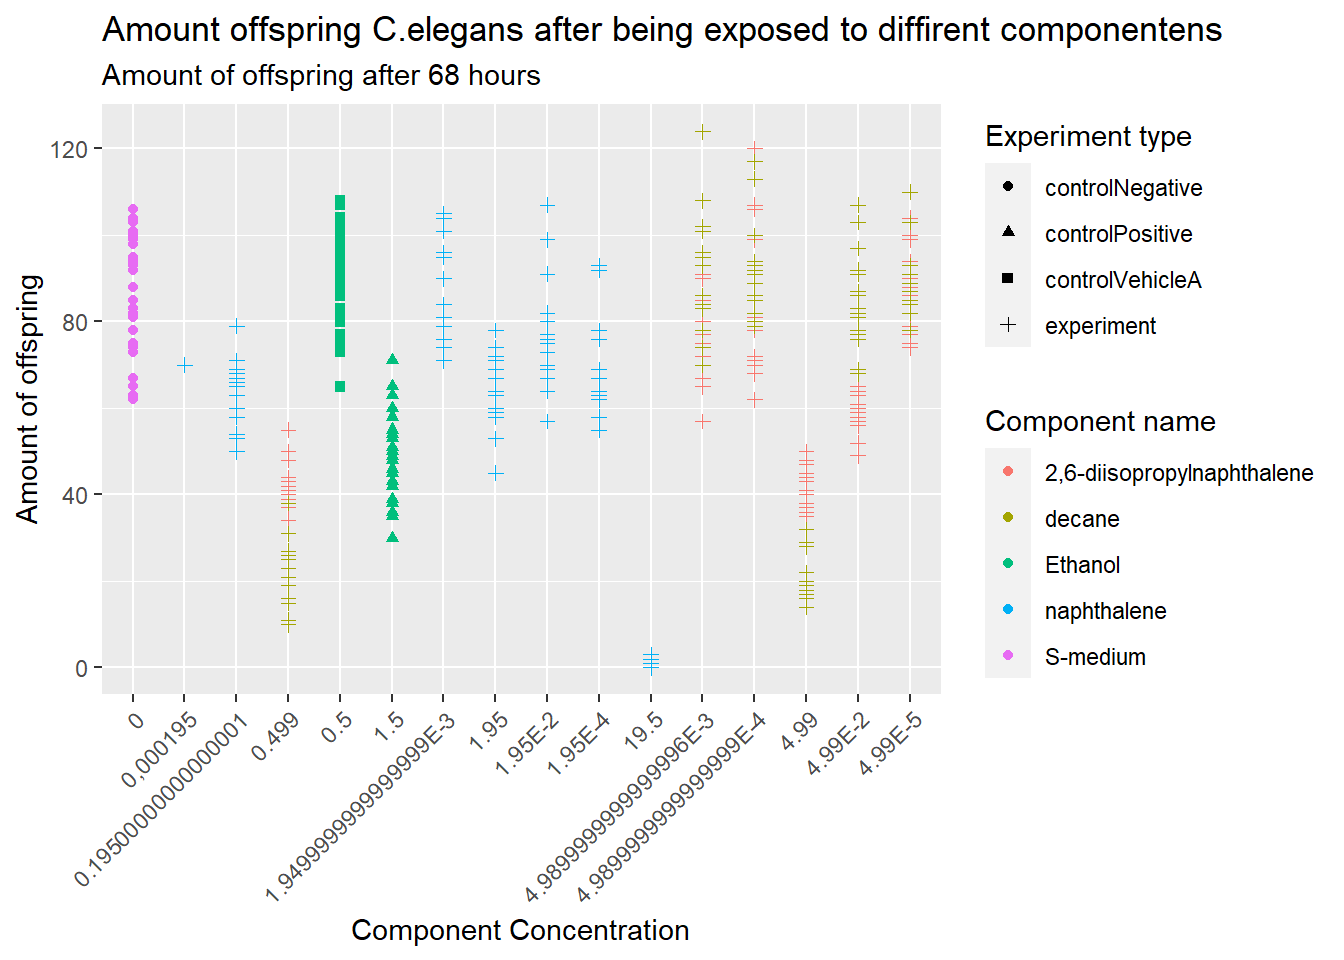
\includegraphics{bookdown-portfolio_files/figure-latex/scatterplot-1.pdf}

\#E. When creating the plot under C), what happened with the ordering of the x-axis labels. Explain why this happens. Look at the data-type of the compConcentration column in the data again to find a clue.
\#\#De volgorde wordt gegroepeerd en niet meer van klein naar groot. Dit komt omdat hij het ziet als characters en dus op alfabetische volgorde zet. 4.99E-5 komt later in het alfabet dat 4.99 en 4 komt later dan 0 of 1

\begin{Shaded}
\begin{Highlighting}[]
\NormalTok{elegansData}\SpecialCharTok{$}\NormalTok{compConcentration }\OtherTok{\textless{}{-}} \FunctionTok{as.numeric}\NormalTok{(elegansData}\SpecialCharTok{$}\NormalTok{compConcentration)}
\end{Highlighting}
\end{Shaded}

\begin{verbatim}
## Warning: NAs introduced by coercion
\end{verbatim}

\#F. Correct this and than look at the graph again.

\begin{Shaded}
\begin{Highlighting}[]
  \FunctionTok{ggplot}\NormalTok{(elegansData, }\FunctionTok{aes}\NormalTok{(}\AttributeTok{x=}\NormalTok{compConcentration, }\AttributeTok{y=}\NormalTok{RawData, }\AttributeTok{shape=}\NormalTok{expType, }\AttributeTok{colour=}\NormalTok{compName, }\AttributeTok{label=}\FunctionTok{round}\NormalTok{(compConcentration, }\AttributeTok{digits =} \DecValTok{3}\NormalTok{)))}\SpecialCharTok{+}
  \FunctionTok{geom\_point}\NormalTok{()}\SpecialCharTok{+}
  \FunctionTok{labs}\NormalTok{(}\AttributeTok{colour=}\StringTok{"Component naam"}\NormalTok{, }\AttributeTok{shape=}\StringTok{"Experiment type"}\NormalTok{,}
       \AttributeTok{x=}\StringTok{"Component Concentratie"}\NormalTok{,}
       \AttributeTok{y=}\StringTok{"Aantal nakomelingen"}\NormalTok{,}
       \AttributeTok{title=}\StringTok{"Aantal nakomelingen C.elegans na bloodstelling met verschillende componenten"}\NormalTok{,}
       \AttributeTok{subtitle=} \StringTok{"Aantal nakomelingen na 68 uur"}
\NormalTok{)}
\end{Highlighting}
\end{Shaded}

\begin{verbatim}
## Warning: Removed 6 rows containing missing values (`geom_point()`).
\end{verbatim}

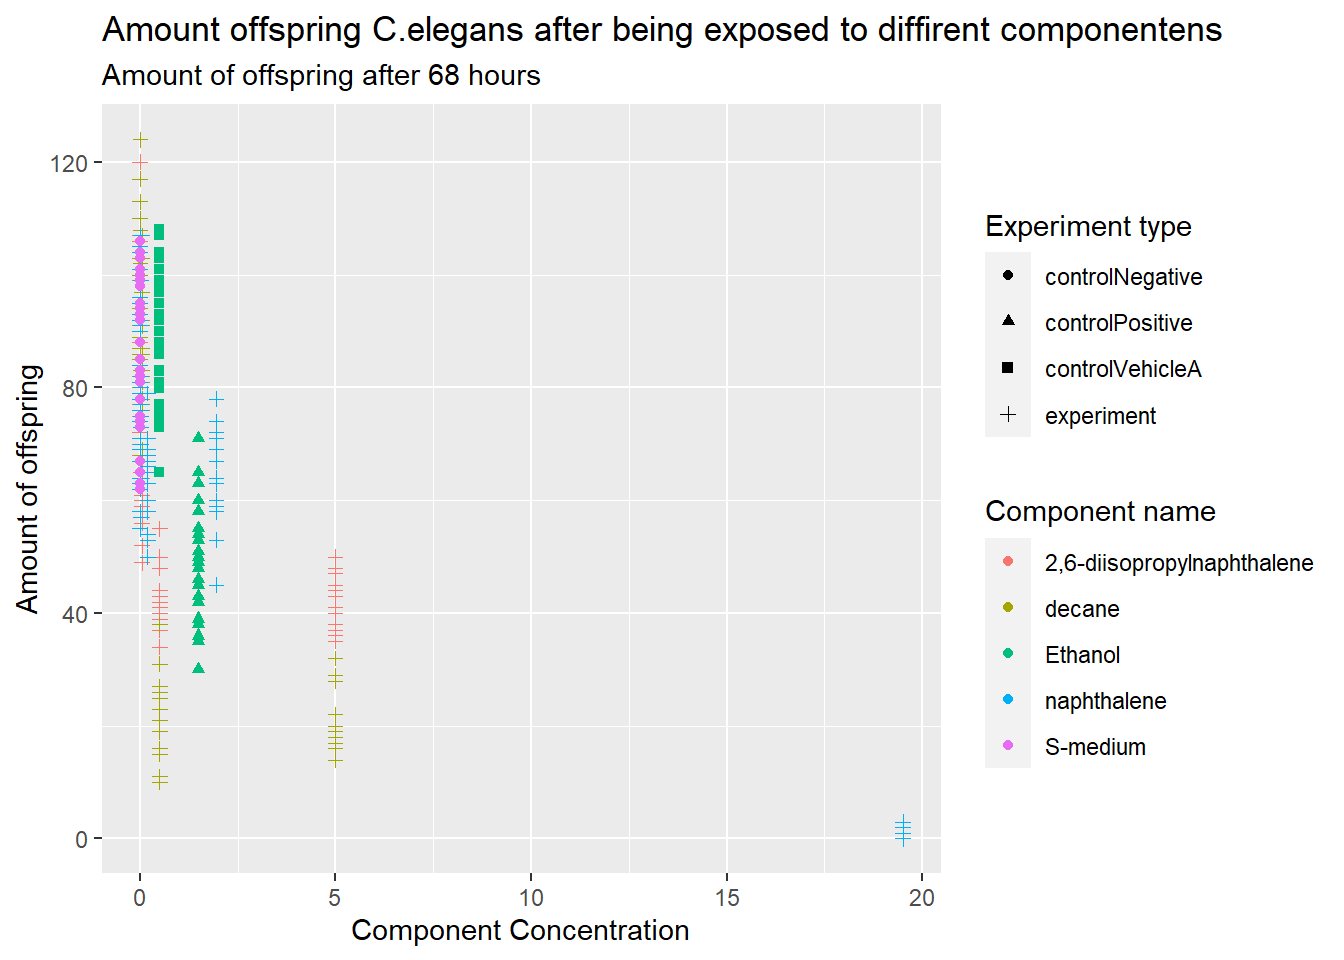
\includegraphics{bookdown-portfolio_files/figure-latex/scatterplot after compC is numeric-1.pdf}

\#F.2 Use a log10 transformation on the x-axis to get a clear graph. Also, add a bit of jitter to the points in the graph so that points are not overlapping (Google ``ggplot jitter'' if needed).

\begin{Shaded}
\begin{Highlighting}[]
\NormalTok{elegansData\_nM }\OtherTok{\textless{}{-}}\NormalTok{ elegansData }\SpecialCharTok{\%\textgreater{}\%} \FunctionTok{filter}\NormalTok{(compUnit }\SpecialCharTok{==} \StringTok{"nM"}\NormalTok{)}

  \FunctionTok{ggplot}\NormalTok{(elegansData\_nM, }\FunctionTok{aes}\NormalTok{(}\AttributeTok{x=}\FunctionTok{log10}\NormalTok{(compConcentration), }\AttributeTok{y=}\NormalTok{RawData, }\AttributeTok{colour=}\NormalTok{compName))}\SpecialCharTok{+}
  \FunctionTok{geom\_point}\NormalTok{(}\AttributeTok{position =} \FunctionTok{position\_jitter}\NormalTok{(}\AttributeTok{h=}\FloatTok{0.15}\NormalTok{,}\AttributeTok{w=}\FloatTok{0.15}\NormalTok{))}\SpecialCharTok{+}
  \FunctionTok{scale\_x\_continuous}\NormalTok{()}\SpecialCharTok{+}
  \FunctionTok{labs}\NormalTok{(}\AttributeTok{colour=}\StringTok{"Component naam"}\NormalTok{,}
       \AttributeTok{x=}\StringTok{"log10 Concentratie(nM)"}\NormalTok{,}
       \AttributeTok{y=}\StringTok{"Aantal nakomelingen"}\NormalTok{,}
       \AttributeTok{title=}\StringTok{"Aantal nakomelingen C.elegans na bloodstelling met verschillende componenten"}\NormalTok{,}
       \AttributeTok{subtitle=} \StringTok{"Aantal nakomelingen na 68 uur"}
\NormalTok{)}\SpecialCharTok{+}
  \FunctionTok{facet\_wrap}\NormalTok{(}\SpecialCharTok{\textasciitilde{}}\NormalTok{compName)}
\end{Highlighting}
\end{Shaded}

\begin{verbatim}
## Warning: Removed 6 rows containing missing values (`geom_point()`).
\end{verbatim}

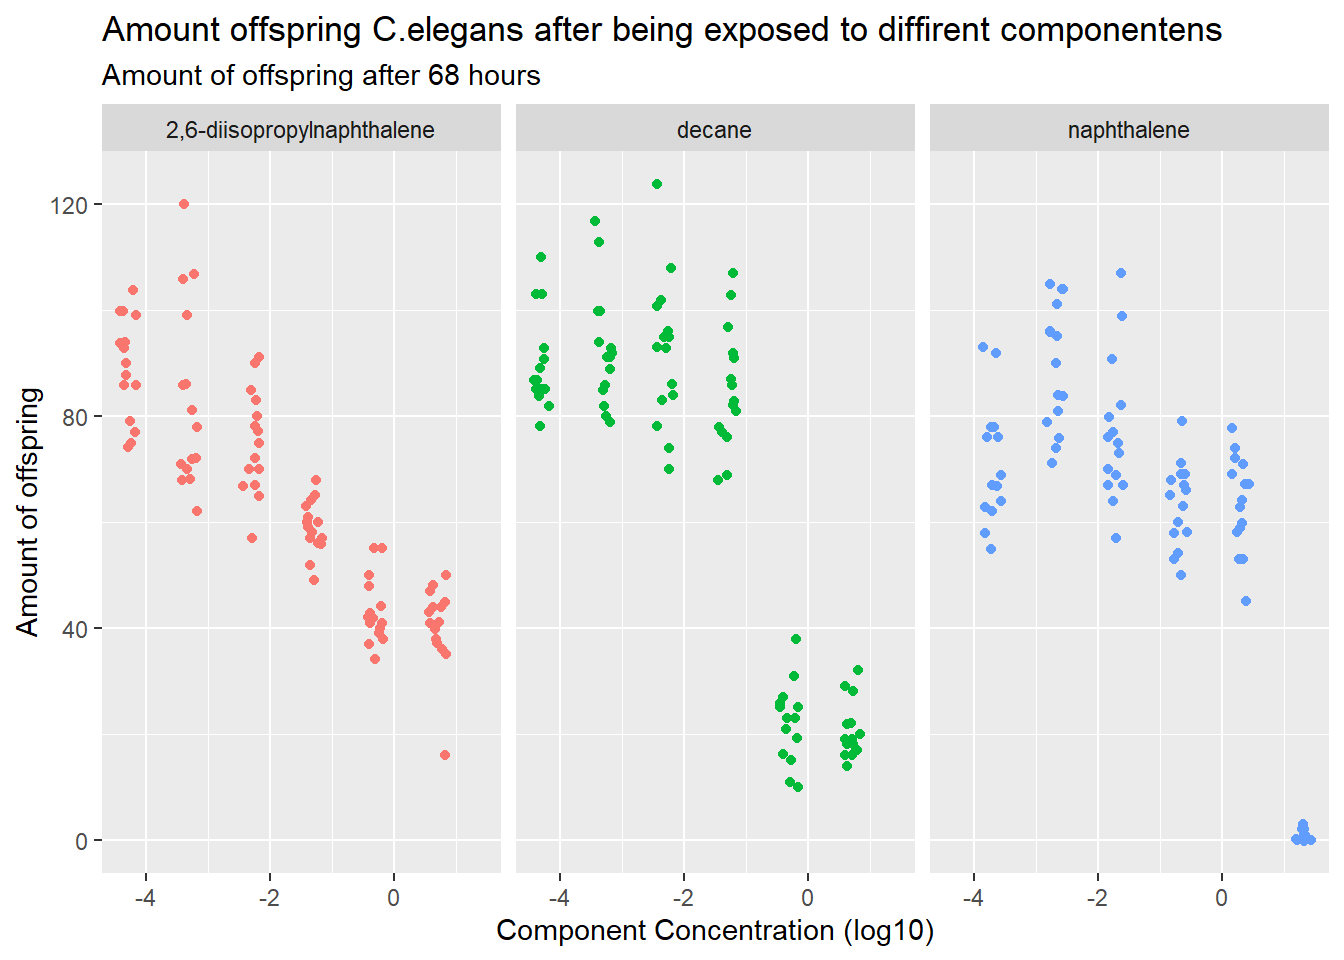
\includegraphics{bookdown-portfolio_files/figure-latex/scatterplot jitter-1.pdf}

\begin{Shaded}
\begin{Highlighting}[]
\NormalTok{elegansData\_pct }\OtherTok{\textless{}{-}}\NormalTok{ elegansData }\SpecialCharTok{\%\textgreater{}\%} \FunctionTok{filter}\NormalTok{(compUnit }\SpecialCharTok{==} \StringTok{"pct"}\NormalTok{)}

\FunctionTok{ggplot}\NormalTok{(elegansData\_pct, }\FunctionTok{aes}\NormalTok{(}\AttributeTok{x=}\NormalTok{compConcentration, }\AttributeTok{y=}\NormalTok{RawData, }\AttributeTok{shape=}\NormalTok{expType, }\AttributeTok{colour=}\NormalTok{compName))}\SpecialCharTok{+}
  \FunctionTok{geom\_point}\NormalTok{(}\AttributeTok{position =} \FunctionTok{position\_jitter}\NormalTok{(}\AttributeTok{h=}\FloatTok{0.1}\NormalTok{,}\AttributeTok{w=}\FloatTok{0.1}\NormalTok{))}\SpecialCharTok{+}
  \FunctionTok{coord\_cartesian}\NormalTok{(}\AttributeTok{ylim =} \FunctionTok{c}\NormalTok{(}\DecValTok{0}\NormalTok{, }\DecValTok{120}\NormalTok{))}\SpecialCharTok{+}
  \FunctionTok{labs}\NormalTok{(}\AttributeTok{colour=}\StringTok{"Component"}\NormalTok{, }\AttributeTok{shape=}\StringTok{"Experiment type"}\NormalTok{,}
       \AttributeTok{x=}\StringTok{"Concentratie in procenten"}\NormalTok{,}
       \AttributeTok{y=}\StringTok{"Aantal nakomelingen"}\NormalTok{,}
       \AttributeTok{title=}\StringTok{"Aantal nakomelingen C.elegans na bloodstelling met verschillende componenten"}\NormalTok{,}
       \AttributeTok{subtitle=} \StringTok{"Aantal nakomelingen na 68 uur"}
\NormalTok{)}
\end{Highlighting}
\end{Shaded}

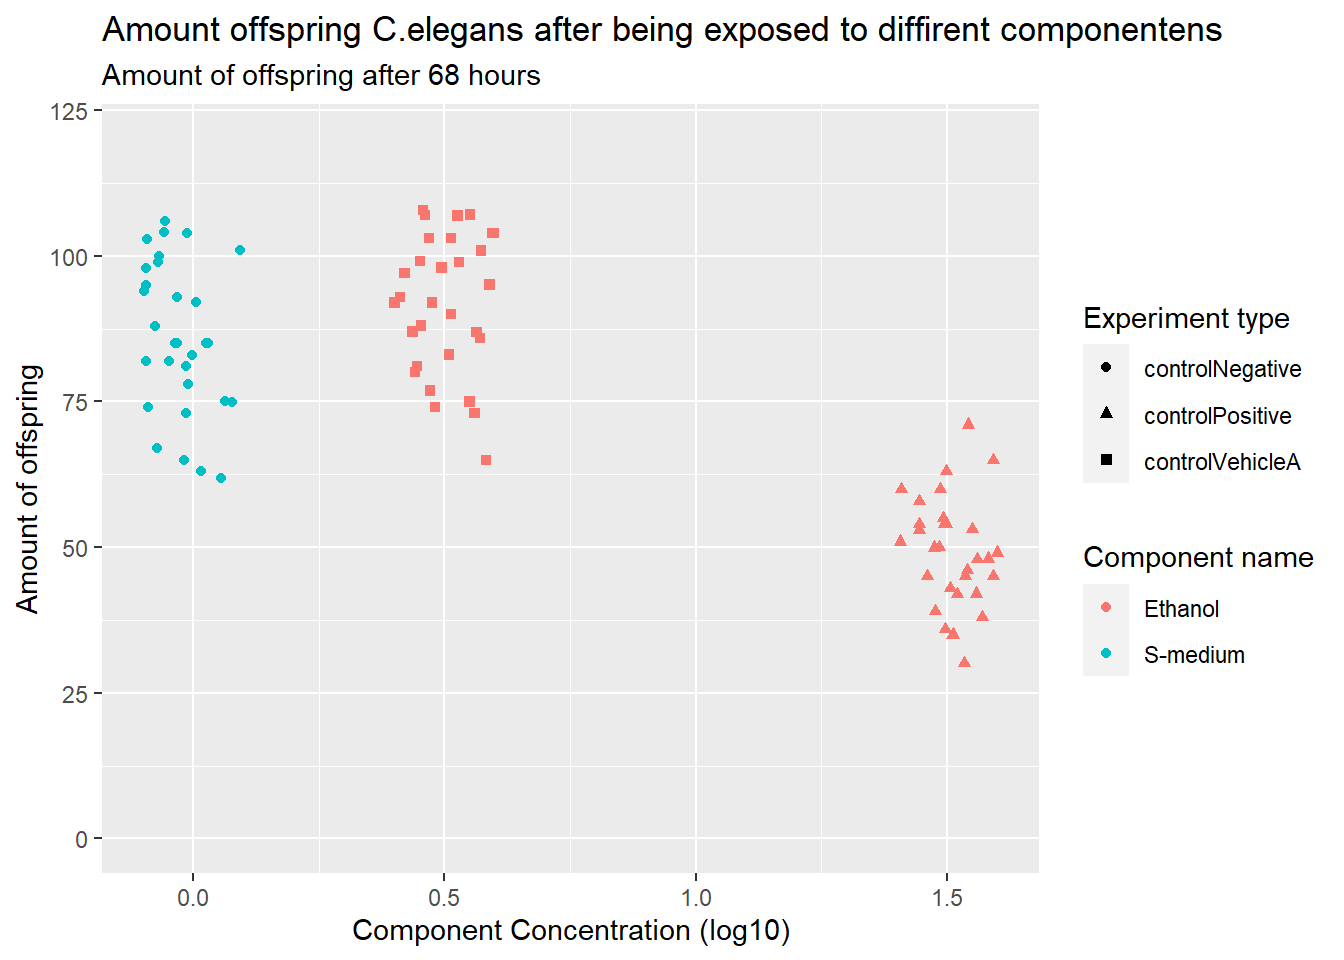
\includegraphics{bookdown-portfolio_files/figure-latex/scatterplot jitter-2.pdf}

\#Fill in:
\#\#(G) The positive control for this experiments is ethanol (expType controlPositive).
\#\#(H) The negative control for this experiment is s-medium (expType controlNegative).

\#I. Think about how you would analyze this experiment to learn whether there is indeed an effect of different concentrations on offspring count and whether the different compounds have a different curve (IC50). Write down you analysis as a step-wise plan.

\#J. Normalize the data for the controlNegative in such a way that the mean value for controlNegative is exactly equal to 1 and that all other values are expressed as a fraction thereof. Rerun your graphs with the normalized data.

\#K. Why would you want to take the step under J?

\end{document}
